\documentclass{article}
\usepackage{graphicx} % Required for inserting images
\usepackage{amsmath}
\usepackage{amssymb}
\usepackage{float}
\usepackage{textgreek}
\usepackage{fancyhdr}
\usepackage{hyperref}

% vnořené popisky obrázků
\usepackage{subcaption}

% automatická konverze EPS 
\usepackage{graphicx} 
\usepackage{epstopdf}

\pagestyle{fancy}


\newcommand\mat[1]{\begin{bmatrix}#1\end{bmatrix}}
\newcommand\pdiff[2]{\frac{\partial #1}{\partial #2}}
\newcommand\hw[1]{\stepcounter{section}\section*{Úkol \thesection\quad #1}}

\title{ARI-HW\_09}
\author{Matěj Pinkas}
\date{20. April 2024}


\lhead{Pinkas Matěj}
\chead{ARI-HW\_09}
\rhead{20. April 2024}

\begin{document}

\maketitle

\section{Příklad}
\subsection{Zadání}
\begin{itemize}
    \item[-] Z datumu narození 10.1.2003 si zvolím konstanty: $d=1$; $m=1$; $r=2$
    \item[-] Konstanty dosadím do zadané rovnice:

    \begin{align*}
        (dr+(d+r)s+s^2)x(s)+(d+s)y(s) &= (d^2+mrd)+(m(d+r)+dr)s+(d+m+r-1)s^2+s^3\\
        (2+(1+2)s+s^2)x(s)+(1+s)y(s) &= (1^2+2)+(1(1+2)+2)s+(1+1+2-1)s^2+s^3\\
        (2+3s+s^2)x(s)+(1+s)y(s) &= 3+5s+3s^2+s^3
    \end{align*}
    \item[-] Z upravené rovnice získám polynomy:
    \begin{align*}
        a(s) &= s^2+3s+2\\
        b(s) &= s+1\\
        c(s) &= s^3+3s^2+5s+3
    \end{align*}
    \item[-] Obecně si za x(s) a y(s) můžu zvolit polynom prvního stupně a dosadit to rovnice:
    \begin{align*}
        x(s) = x_0 + sx_1\\
        y(s) = y_0 + sy_1\\
        (2+3s+s^2)(x_0 + sx_1)+(1+s)(y_0 + sy_1) &= 3+5s+3s^2+s^3\\
    \end{align*}
    \item[-] Z výsledného polynomu vytvořím Sylvestrovu matici:
    \begin{align*}
        \mat{x_0 & y_0 & x_1 & y_1} \mat{2 & 3 & 1 & 0\\ 1 & 1 & 0 & 0\\ 0 & 2 & 3 & 1\\ 0 & 1 & 1 & 0} = \mat{3 & 5 & 3 & 1}
    \end{align*}

    \item[-] Vytvořím si soustavu rovnic ze Sylvestrovy matice a vyřeším pro neznáme $x_0$, $y_0$, $x_1$, $y_1$:
    \begin{align*}
        a_0x_0+b_0y_0 &= c_0\\
        a_1x_0+b_1y_0+a_0x_1+b_0y_1 &= c_1\\
        a_2x_0+b_2y_2+a_1x_1+b_1y_1 &= c_2\\
        a_2x_1+b_2y_1 &= c_3
    \end{align*}
    
    \begin{align*}
        2x_0+1y_0 &= 3\\
        3x_0+1y_0+2x_1+1y_1 &= 5\\
        1x_0+0y_2+3x_1+1y_1 &= 3\\
        1x_1+0y_1 &= 1
    \end{align*}
    
    \begin{align*}
        2x_0+y_0 &= 3\\
        3x_0+y_0+2x_1+y_1 &= 5\\
        x_0+3x_1+y_1 &= 3\\
        x_1 &= 1
    \end{align*}
    
    \begin{align*}
        x_0 &= 0 & y_0 &= 3 & x_1 &= 1 & y_1 &= 0\\
    \end{align*}
    \item[-] Získané $x_0$, $y_0$, $x_1$, $y_1$ dosadím do zvolených $x(s)$ a $y(s)$:
    \begin{align*}
        x(s) = x_0 + sx_1 = 0 + 1s = s\\
        y(s) = y_0 + sy_1 = 3 + 0s = 3
    \end{align*}

    \item[-] Metodou redukce pokračuji: 

    \begin{align*}
        \mat{a(s) & 1 & 0\\ b(s) & 0 & 1} = \mat{s^2+3s+2 & 1 & 0\\s+1 & 0 & 1} &=  \mat{(s+2)(s+1) & 1 & 0\\s+1 & 0 & 1} = \mat{0 & 1 & -(s+2)\\s+1 & 0 & 1} \\ &= \mat{s+1 & 0 & 1\\0 & 1 & -s-2} = \mat{g(s) & p(s) & q(s)\\ 0 & v(s) & w(s)}
    \end{align*}
    
    \begin{align*}
        \overline{c}(s) = \frac{c(s)}{g(s)} = \frac{s^3+3s^2+5s+3}{s+1} = \frac{(s+1)(s^2+2s+3)}{s+1} = s^2+2s+3
    \end{align*}
    
    \begin{align*}
        x(s) &= p(s)\overline{c}(s) = 0\\
        y(s) &= q(s)\overline{c}(s) = s^2+2s+3
    \end{align*}
    
    \begin{align*}
        x(s) &= p(s)\overline{c}(s) + v(s)t(s) = 0+t(s)\\
        y(s) &= q(s)\overline{c}(s) + w(s)t(s) = s^2+2s+3-(s+2)t(s)
    \end{align*}
    
    \begin{align*}
        t(s) &= 0 \Rightarrow & x(s) &= 0 & y(s) &= s^2+2s+3\\
        t(s) &= s \Rightarrow & x(s) &= s & y(s) &= 3
    \end{align*}

    \subsection{Řešení minimálního stupně x}
    \item[-] Po dosazení t(s)=0 do funce:
    \[x(s) = 0+t(s) \Rightarrow x(s) = 0\]
    \item[] získám očividně nejnižší stupeň v x, zbytkem partikulárního řešení je:\\
    \[y(s)= s^2+2s+3\]
    
    \subsection{Řešení minimálního stupně y}
    \item[-] Nejdříve zjistím jakého stupně bude $\overline{a}$
    \begin{align*}
        deg_y &= deg(y(s)) = deg(3) = 0\\
        \overline{a}(s) &= \frac{a(s)}{g(s)} = \frac{s^2+3s+2}{s+1} = \frac{(s+2)(s+1)}{s+1} = s+2\\
        deg_{\overline{a}} &= deg(\overline{a}(s)) = deg(s+2) = 1
    \end{align*}
    \item[-] nyní díky podmínce, že $deg(y) < deg(\overline{a})$ 
    \item[-] opravdu tedy mohu dosadit t(s)=s a získám řešení:
    \[x(s) = s\]
    \[y(s) = 3\]
    \item[] $deg(y) = 0 < deg(\overline{a}) = 1 \Rightarrow$ tato podmínka platí, tak mohu uznat tento polynom za minimální 
    
    
    \subsection{Funkce axbyc()}
    \item[-] Pomocí funkce $axbyc()$ z toolboxu PolX získám minimální hodnotu\\ v $x$ a $y$:
    \begin{align*}
        axbyc(a(s),b(s),c(s),'minx') & \Rightarrow & x(s) &= 0 & y(s) &= s^2+2s+3\\
        axbyc(a(s),b(s),c(s),'miny') & \Rightarrow & x(s) &= s & y(s) &= 3
    \end{align*}
    
    \item[] ještě získám celkové minimální polynomy x a y
    \begin{align*}
        axbyc(a(s),b(s),c(s),'syl') & \Rightarrow & x(s) &= s+1 & y(s) &= 1-s
    \end{align*}
    
\end{itemize}




\section{Příklad}

\begin{itemize}
    \item[] Zadaný systém: 
    \begin{align*}
        \frac{b(s)}{a(s)} = \frac{s+2}{s(s-1)}
    \end{align*}

    \subsection{}
    \item[-] Nejdříve zjistím omezení na stupeň polynomu c(s):
    \begin{align*}
        deg(a(s)) &= 2\\
        deg(c(s)) &\ge 2deg(a(s))-1 = 3\\
        &\Rightarrow deg(c(s)) \ge 3
    \end{align*}

    \item[-] Nyní charakteristický polynom napíšu ze zadání a přidám pól pro vykrácení nuly: 
    \begin{align*}
        c(s) &= (s+2+j)(s+2-j)\\
        c(s) &= (s+2+j)(s+2-j)(s+2)
    \end{align*}
    \item[-] c(s) stále splňuje podmínku stupně nižší rovno 3 

    \item[-] Obecné polynomy obecného regulátoru tedy vypadají takto: 
    \begin{align*}
        c(s) = a(s)p(s)+b(s)q(s)\\
        c(s) = f(s)t(s)+b(s)r(s)
    \end{align*}

    \item[-] Po nalezení partikulárního řešení pomocí funkce $axbyc()$ získám polynomy: 
    \begin{align*}
        p(s) &= 2 + s\\
        q(s) &= 5 + 5s\\
        r(s) &= 5 + 4s
    \end{align*}

    \subsection{}
    \item[-] Přenos celé soustavy T(s) tedy je:
    \begin{align*}
        T(s) = \frac{b(s)r(s)}{a(s)p(s)+b(s)q(s)} = \frac{(4 s + 5) (s + 2)}{(5 s + 5) (s + 2) + s (s - 1) (s + 2)} = \frac{4 s^2 + 13 s + 10}{s^3 + 6 s^2 + 13 s + 10}
    \end{align*}

    \subsection{}
    \begin{figure}[H]
        \centering
        \begin{subfigure}[b]{0.45\textwidth}
            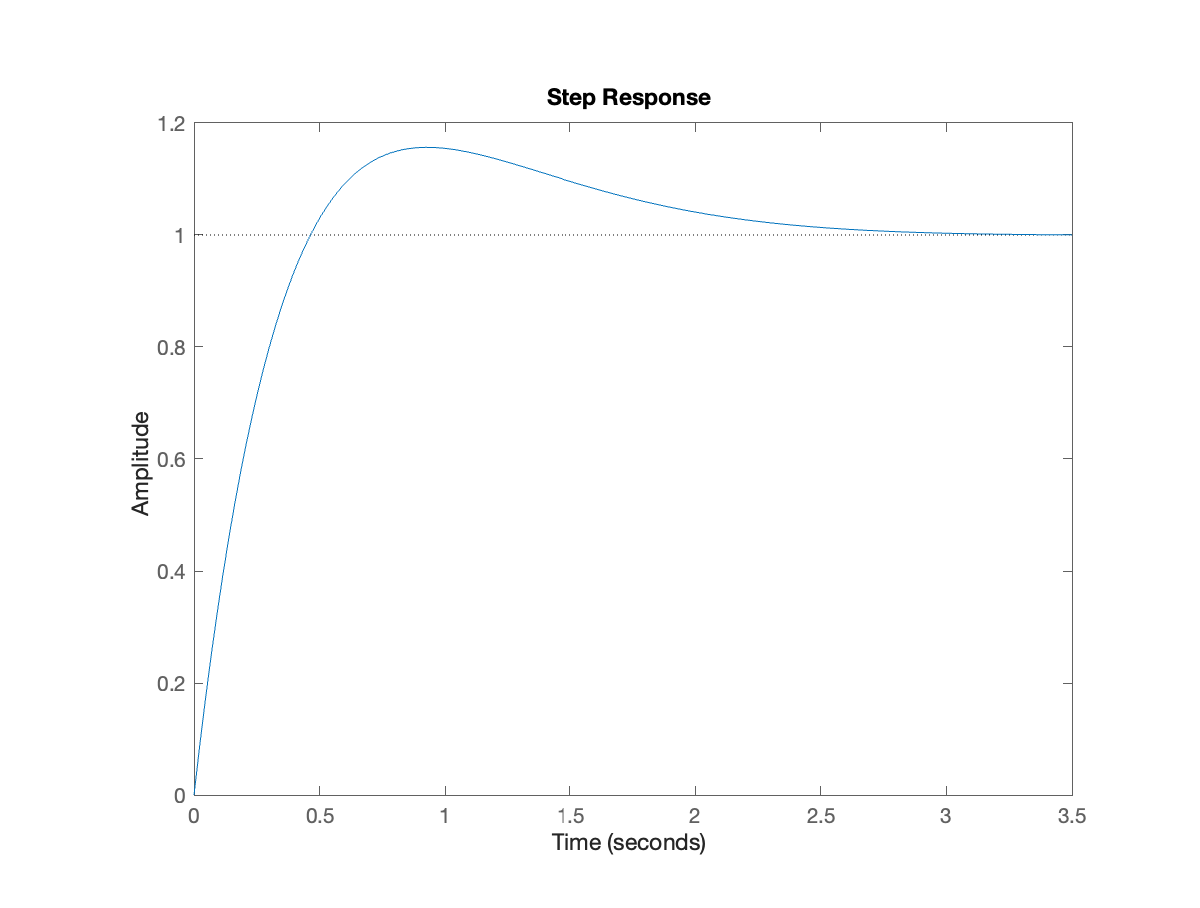
\includegraphics[width=\textwidth]{Step_response.eps}
            \caption{Odezva T(s) na skok}
            \label{fig:Step_response}
        \end{subfigure}
        ~
        \begin{subfigure}[b]{0.45\textwidth}
            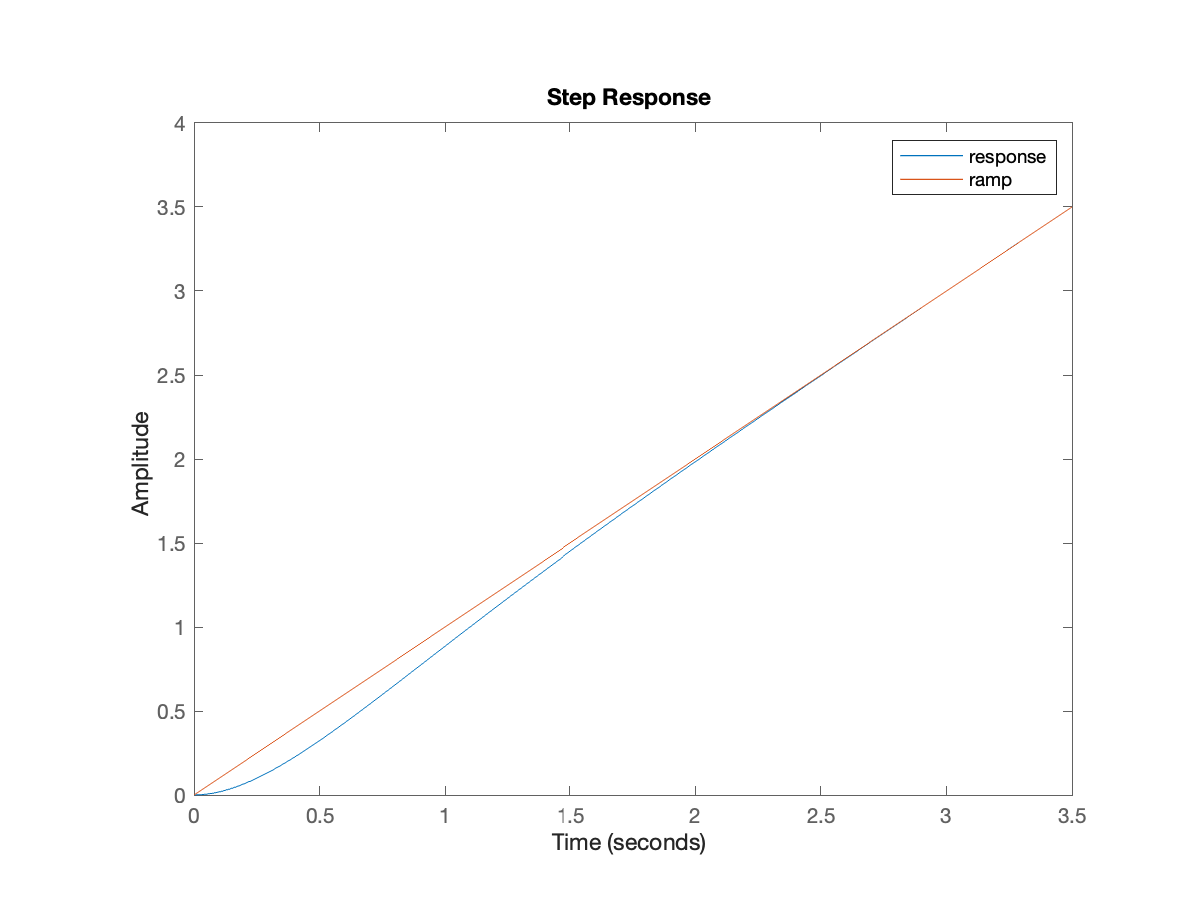
\includegraphics[width=\textwidth]{ramp_response.eps}
            \caption{Odezva T(s) na rampu}
            \label{fig:Ramp_response}
        \end{subfigure}
     
        \label{fig:13cIICompare}
    \end{figure}
    
\end{itemize}


\end{document}
